\documentclass[tikz,border=5pt]{standalone}
\usepackage[T1]{fontenc}
\usepackage{lmodern,amsmath,amssymb}
\usetikzlibrary{arrows.meta,calc,positioning,fit,backgrounds,shapes.geometric,matrix,decorations.pathreplacing,patterns}
\definecolor{ink}{gray}{0.08}
\definecolor{wash}{gray}{0.965}
\definecolor{soft}{gray}{0.45}
\tikzset{box/.style={draw=ink,line width=.65pt,fill=white,align=center,inner sep=4pt,outer sep=0pt,font=\small},flow/.style={draw=ink,line width=.65pt,-{Latex[length=1.8mm,width=1.3mm]},rounded corners=2pt},annotation/.style={font=\scriptsize,text=soft,align=center},groupbox/.style={draw=soft,dashed,line width=.45pt,fill=wash}}
\begin{document}
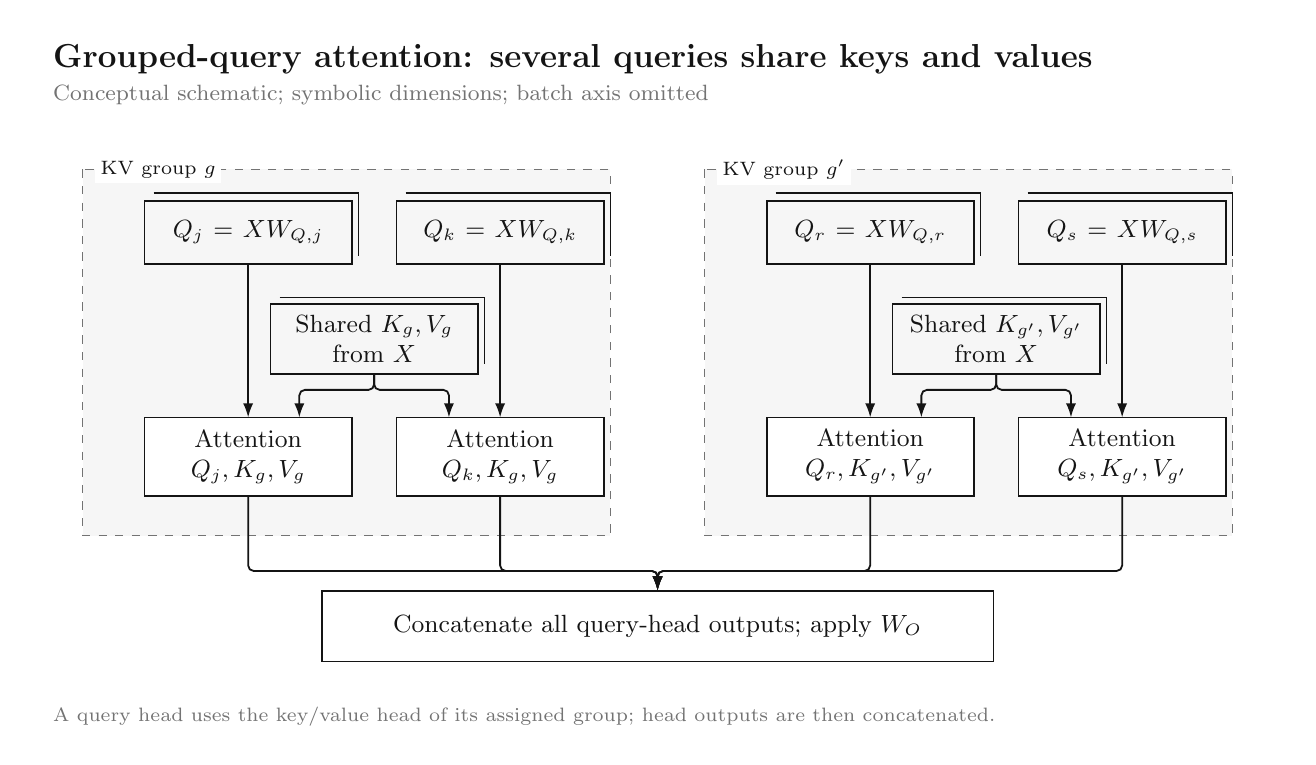
\begin{tikzpicture}[x=1cm,y=-1cm,font=\rmfamily,text=ink]

\path[use as bounding box] (0,0) rectangle (16,9);
\node[anchor=west,font=\large\bfseries] at (.2,.4) {Grouped-query attention: several queries share keys and values};
\node[anchor=west,font=\footnotesize,text=soft] at (.2,.85) {Conceptual schematic; symbolic dimensions; batch axis omitted};
\begin{pgfonlayer}{background}
\draw[groupbox] (0.7,1.8) rectangle (7.4,6.45);
\node[anchor=west,font=\scriptsize,fill=white,inner sep=2pt] at (0.85,1.8) {KV group $g$};
\draw[groupbox] (8.6,1.8) rectangle (15.3,6.45);
\node[anchor=west,font=\scriptsize,fill=white,inner sep=2pt] at (8.75,1.8) {KV group $g'$};
\end{pgfonlayer}
\node[box,fill=wash,minimum width=2.6cm,minimum height=0.8cm,text width=2.35cm] (qj) at (2.8,2.6) {$Q_{j}=XW_{Q,j}$};
\draw[ink,line width=.4pt] (1.5999999999999999,2.1) -- (4.199999999999999,2.1) -- (4.199999999999999,2.9);
\node[box,minimum width=2.6cm,minimum height=1.0cm,text width=2.35cm] (aj) at (2.8,5.45) {Attention\\$Q_{j},K_{g},V_{g}$};
\node[box,fill=wash,minimum width=2.6cm,minimum height=0.8cm,text width=2.35cm] (qk) at (6.0,2.6) {$Q_{k}=XW_{Q,k}$};
\draw[ink,line width=.4pt] (4.8,2.1) -- (7.3999999999999995,2.1) -- (7.3999999999999995,2.9);
\node[box,minimum width=2.6cm,minimum height=1.0cm,text width=2.35cm] (ak) at (6.0,5.45) {Attention\\$Q_{k},K_{g},V_{g}$};
\node[box,fill=wash,minimum width=2.6cm,minimum height=0.85cm,text width=2.35cm] (kvj) at (4.4,3.95) {Shared $K_{g},V_{g}$\\from $X$};
\draw[ink,line width=.4pt] (3.2000000000000006,3.4250000000000003) -- (5.8,3.4250000000000003) -- (5.8,4.275);
\node[box,fill=wash,minimum width=2.6cm,minimum height=0.8cm,text width=2.35cm] (qr) at (10.7,2.6) {$Q_{r}=XW_{Q,r}$};
\draw[ink,line width=.4pt] (9.499999999999998,2.1) -- (12.1,2.1) -- (12.1,2.9);
\node[box,minimum width=2.6cm,minimum height=1.0cm,text width=2.35cm] (ar) at (10.7,5.45) {Attention\\$Q_{r},K_{g'},V_{g'}$};
\node[box,fill=wash,minimum width=2.6cm,minimum height=0.8cm,text width=2.35cm] (qs) at (13.9,2.6) {$Q_{s}=XW_{Q,s}$};
\draw[ink,line width=.4pt] (12.7,2.1) -- (15.3,2.1) -- (15.3,2.9);
\node[box,minimum width=2.6cm,minimum height=1.0cm,text width=2.35cm] (as) at (13.9,5.45) {Attention\\$Q_{s},K_{g'},V_{g'}$};
\node[box,fill=wash,minimum width=2.6cm,minimum height=0.85cm,text width=2.35cm] (kvr) at (12.3,3.95) {Shared $K_{g'},V_{g'}$\\from $X$};
\draw[ink,line width=.4pt] (11.1,3.4250000000000003) -- (13.700000000000001,3.4250000000000003) -- (13.700000000000001,4.275);
\node[box,minimum width=8.5cm,minimum height=0.9cm,text width=8.25cm] (cat) at (8,7.6) {Concatenate all query-head outputs; apply $W_O$};
\begin{pgfonlayer}{background}
\draw[flow] (qj.south) -- (aj.north);
\draw[flow] (qk.south) -- (ak.north);
\draw[flow] (qr.south) -- (ar.north);
\draw[flow] (qs.south) -- (as.north);
\draw[flow] (aj.south) -- (2.8,6.9) -- (8,6.9) -- (cat.north);
\draw[flow] (ak.south) -- (6,6.9) -- (8,6.9) -- (cat.north);
\draw[flow] (ar.south) -- (10.7,6.9) -- (8,6.9) -- (cat.north);
\draw[flow] (as.south) -- (13.9,6.9) -- (8,6.9) -- (cat.north);
\end{pgfonlayer}
\draw[flow] (kvj.south)--(4.4,4.6)--(3.4499999999999997,4.6)--(3.4499999999999997,4.95);
\draw[flow] (kvj.south)--(4.4,4.6)--(5.35,4.6)--(5.35,4.95);
\draw[flow] (kvr.south)--(12.3,4.6)--(11.35,4.6)--(11.35,4.95);
\draw[flow] (kvr.south)--(12.3,4.6)--(13.25,4.6)--(13.25,4.95);
\node[anchor=west,align=left,font=\scriptsize,text=soft,text width=15.6cm] at (.2,8.75) {A query head uses the key/value head of its assigned group; head outputs are then concatenated.};
\end{tikzpicture}
\end{document}
